\chapter{Incremental Dense Refinement}
\label{ch:incrDenseRef}
The reconstruction methods described thus far, build a manifold mesh from a set of sparse data. 
The outcome is able to capture the coarse geometry of the mesh, and even after the mesh sweeping, the reconstruction still lacks to capture the fine-grained details.
In this chapter we aim at recovering the details of the geometry of the scene, incrementally, by means of variational optimization which directly evolves the surface of the scene according to images. 
We present a fully automatic pipeline to incrementally estimate the accurate reconstruction. In particular the method described is able to handle multi-resolution mesh: instead of merging accurate submaps of the scene a-posteriori and off-line, it combines directly online the reconstruction refined with the variational algorithm together with the new rough manifold estimated with the algorithms presented in the previous chapters.

\minitoc

\section{Rationale}

Classical Multi-View Stereo methods \cite{gargallo2005bayesian,delaunoy_et_al_08} handle small objects, e.g., those proposed in the benchmark of Stretcha \etal \cite{strecha2006combined}.
The reasons are related both to the computational and memory resources needed to handle big set of images, and to the limitations of the optimization procedures.
The common volumetric voxel-based representation of the space requires a huge amount of memory to store accurate and detailed data.
Thanks to the introduction of hashing methods and especially  Delaunay Triangulation based methods, algorithms to deal with large-scales scenes have been proposed.
Successful Delaunay-based incremental approaches have been proposed in \cite{lovi_et_al_11,hoppe2013incremental,litvinov_lhuillier_13,romanoni15b,romanoni15a} but they all rely sparse data and visibility-only information, therefore the final reconstruction lacks in details and is not photo-consistent.


A very popular class of  incremental dense reconstruction algorithms relies on depth maps; they first estimate the depth map for a selected set of keyframe, then they merge the depth maps into a single consistent 3D model of the scene. 
Most of the depth maps-based approaches \cite{pollefeys_et_al_08,collins1996space,newcombe2010live,ohtake2003multi,stuhmer2012parallel,stuckler2014multi} rely on a voxel-based volumetric representation of the TSDF and are not suitable for large-scale reconstruction. 
Sch{\"o}ps \etal \cite{schops20153d} propose then to use voxel hashing together with a careful filtering of noisy depth data.
Even if the results are remarkable, the resulting model is a non-continuous mesh, and the meshing step is not directly driven by the images, but by marching cubes \cite{lorensen1987marching} that interpolates the TSDF , as in most of the depth map based approaches.

Mesh-based algorithms represent an effective alternative to depth-maps based reconstruction. Labatut \etal \cite{labatut2007efficient} estimate directly a visibility and photo-consistent mesh from the Delaunay triangulation of the 3D noisy points obtained from the depth maps.
Vu \etal  \cite{vu_et_al_2012} improve this algorithm by estimating an initial visibility-consistent mesh then by evolving the mesh such that it maximizes the photo-consistency with respect to the images. 
These Delaunay-based volumetric approaches are able to handle large scale scenes, but both \cite{labatut2007efficient} and \cite{vu_et_al_2012}  are not incremental.
Moreover, in the remarkable work of Vu \etal \cite{vu_et_al_2012}, the reconstruction pipeline   is not fully automatic, since the optimization method is well suited for 2-manifold meshes, but the method proposed to estimate the initial mesh does not guarantee that manifold property holds for the whole model.



In this chapter we propose a framework to overcome the previous limitation, which is the first incremental algorithm for large-scale environments, which reconstruct a continuous and photo-consistent manifold mesh. 
We propose a fully automatic pipeline that integrates existing works on manifold reconstruction with the accurate surface evolving refinement step and a novel manifold-preserving mesh merging algorithm.


\section{System overview}
 
\section{Proposed system}
 Our approach combines three steps  to provide a fully automatic and incremental reconstruction of the environment, which is photo-consistent with the images. In Fig. \ref{fig:architecture} we illustrate a scheme of the whole system. Every  $W$ frames the system outputs the available reconstruction.
 
 \begin{figure}[t]
  \centering
  \includegraphics[width=0.8\textwidth]{./img/ch-incr-dens/incremental-mvs-architectureNEW}
  \caption{Architecture of the parallel and incremental reconstruction system}
  \label{fig:architecture}
\end{figure}


The first step  incrementally builds a manifold mesh  from Structure from Motion 3D points and camera poses up to time $t$: this output a mesh $\mathit{M}_{0..t}^{\text{rec}}$: therefore,  $\mathit{M}_{0..W}^{\text{rec}}$ is a first rough initialization for the subsequent step. We combine all the subsequent meshes $\mathit{M}_{0..kW}^{\text{rec}}$, with $k>1$ with the refined ones $\mathit{M}_{0..(k-1)W}^{\text{opt}}$. 
In this step we enforce the manifold property in the previous step in order to consistently apply the following mesh evolution process.

The second step is dedicated to the windowed variational refinement of the input mesh: it evolves the surface to maximize the photo-consistency between the last subsequent $W$ pairwise cameras. 
%This approach reaches very accurate results and have been proved to scales well with large-scale scenes \cite{vu2011large}.

In the third step we combine the output of refinement, i.e.,   $\mathit{M}_{0..(k-1)W}^{\text{opt}}$  and the new manifold $\mathit{M}_{0..kW}^{\text{rec}}$ with a novel approach that keeps the manifold property and updates the topology. 
The output of this module is the multi-resolution mesh $\mathit{M}_{0..kW}^{\text{merged}}$.



\subsection{Incremental Manifold Surface Reconstruction}
\label{sec:incremental_manifold}
The first step reconstructs a manifold from sparse 3D points, camera poses and visibility information coming from a generic source, for instance an Incremental Structure from Motion algorithm. 

We adopt the approach presented in \cite{litvinov_lhuillier_13}, with the enhancement proposed in \cite{romanoni15a}. The reconstruction algorithm inherits the philosophy of space carving: we partition the space with the Delaunay triangulation of the 3D sparse points, then rather then marking each tetrahedron with a binary label (matter or free space), we associate  to each tetrahedron a weight which keeps track of the visibility information, i.e., the camera-to-point viewing rays. The final manifold surface is the mesh boundary which contains as much intersected tetrahedra as possible such that the manifoldness is preserved.

\subsection{Incremental photo-consistent refinement}
\label{sec:Incremental_photoconsistent}
After a manifold mesh that represents roughly the observed scene is available, we refine the mesh in order to minimize the photo-metric error between pairwise camera induced by the reconstructed surface. 
The approach adopted in our system is framed into the variational problem of finding a convenient function (the reconstructed surface) in order to  accurately represents the image data.
The calculus of variations of an energy function $E$ induced by a vector field $v$ on a surface $\mathit{S}$, leads to the functional gradient
\begin{equation}
\label{eq::calculus}
 DE(\mathit{S})_v = \left.\frac{\partial E(\mathit{S} + \epsilon v)}{\partial \epsilon} \right|_{\epsilon=0} = \int_{\mathit{S}} \nabla E(x)v(x) dx.
\end{equation}

Our surface refinement algorithms minimize an energy:
\begin{equation}
E = E_{\textrm{photo}} + E_{\textrm{smooth}} ,
\end{equation}
where  $E_{\textrm{photo}}$ represents the energy induced by  the photo-consistency with the images, and $E_{\textrm{smooth}}$ is a prior energy that usually enforce the smoothness of the surface.  


We first describe how we minimize the first term which encodes the photo-consistency.
Let consider two images $I_i$ and $I_j$, and the surface reconstructed $\mathit{S}$. Let $x$ and $\overrightarrow{n}$ be a point on this surface and the corresponding normal. We define a function $err_{I_i, I_j}(x_i)$ as photo-metric similarity measure decreasing when the appearance of two images $I_j$ and $I_i$ around 2D point $x_i$ of image $I_i$.
In the early approach of Faugeras \etal \cite{faugeras2002variational} the energy $E_{\textrm{photo}}$ is integrated on the surface, and becomes:
\begin{equation}
 E_{\textrm{photo}} = \sum_{i,j}\int_{\mathit{S}} v^{\mathit{S}}_{ij}(x) sim_{i,j}(x, \overrightarrow{n}) d\mathit{S}
\end{equation}


In our case we prefer to mimimize  \cite{pons2007multi} the image-based  energy $E_{\textrm{photo}}$ becomes:
\begin{equation}
\label{eq:energy_photo}
  E_{\textrm{photo}} = \sum_{i,j}\int_{\Omega^{\textrm{S}}_{i,j}} err_{I_i, I_{ij}^{\mathit{S}}}(x_i)\textrm{d}x_i = \sum_{i,j} \mathit{M}_{ij}(x)
\end{equation}
where the term $I_{ij}^{\mathit{S}}$ represents the reprojection of the image from the $j$-th camera in the image $i$ through the surface $\mathit{S}$.
(Fig. \ref{fig:cameraproj}).
The reasons to choose the latter energy are twofold: we do not explicilty need to consider the visibility and we directly compare the images in their natural domain.

Classical approaches in computer vision both in surface evolution and in other reconstruction methods, such as voxel-based, optimize the energy over a continuous representation of the surface then they discretize the minimizing flow to evolve the mesh-based representation \cite{pons2007multi,faugeras2002variational}. Recently a more coherent approach shows better results \cite{vu_et_al_2012,delaunoy_et_al_08}: it is named discretize-then-optimize and it directly takes into account the mesh representation during the optimizing procedure. 
Therefore we now accommodate equation \eqref{eq::calculus} in order to take into account that  surface $\mathit{S}$ is represented by a triangular mesh. 
Let $X_i \in \mathbb{R}^3$ be a mesh vertex. The discrete vector field associates for each $i$-th vertex a vector $v_i$ is defined such that $v(x) = \sum_i \phi_i(x) v_i$, where, if $x$ is in the triangle containing $X_i$, then $\phi_i(x)$ is the barycentric coordinates otherwise $\phi_i(x) = 0$.


\begin{figure}[t]
\centering
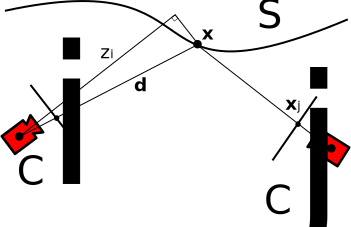
\includegraphics[width=0.5\textwidth]{./img/ch-incr-dens/cameproj}
\label{fig:cameraproj}
\caption{Variables involved in the photometric refinement process}.
\end{figure}

The equation of the gradient functional becomes:
\begin{equation}
  DE(\mathit{S})_v = \sum_i v_i \int_{\mathit{S}} \phi_i(x) \nabla E(x) \textrm{d}x.
\end{equation}

The discrete version of this gradient computed for a single vertex of the mesh becomes:
\begin{equation}
  \frac{\textrm{d}E(\mathit{S})}{\textrm{d}X_i} =  \int_{\mathit{S}} \phi_i(x) \nabla E(x) \textrm{d}x.
\end{equation}

In our case we need to compute the gradient of the energy defined in equation \eqref{eq:energy_photo}:
\begin{equation}
  \nabla E_{\textrm{photo}} = \nabla (\sum_{i,j} err_{ij}(x)) = \sum_{i,j} \nabla err_{ij}(x).
\end{equation}
We suppose the point $x$ projects in points $x^i = \Pi_i(x) \in I_i$ and  $x^j = \Pi_j(x) \in I_j$, then, the vector $\mathbf{d}_i$ goes from camera $i$ to point $x$, $z_i$ is the depth of $x$ in camera $i$, final $\mathbf{N}$ is the normal at $x$ pointing outward the surface $\mathit{S}$. 
Therefore, with the change of variable $\textrm{d}x_i = -\mathbf{N}^T \mathbf{d}_i \textrm{d}x/z_i^3$:
\begin{equation}
  \nabla \mathit{M}_{ij}(x) = -\mathbf{N} \left( \partial_2 err_{I_i, I_{ij}^{\mathit{S}}}(x_i) DI_j(x_j) D\Pi_j(x)\frac{\mathbf{d}_i}{z_i^3}\right) = - f_{ij}(x_i) \mathbf{N}/z_i^3.
\end{equation}
where operator $D$ represents the derivative and $\partial_2 err_{I_i, I_{ij}^{\mathit{S}}}(x_i)$ is the derivative of $err_{ij}(x)$ with respect to the second image.


We then are able to rewrite the discrete gradient:
\begin{equation}
  \frac{\textrm{d}E(\mathit{S})}{\textrm{d}X_i} =  - \int_{\mathit{S}} \phi_i(x) \sum_{i,j} \mathit{M}_{ij}(x) \textrm{d}x 
\end{equation}

\begin{equation}
  =  - \sum_{i,j} \int_{\mathit{S}} \phi_i(x)  f_{ij}(x_i)  \mathbf{N}/z_i^3 \textrm{d}x 
\end{equation}
\begin{equation}
  =  - \sum_{i,j} \int_{\mathit{S}} \phi_i(x)  f_{ij}(x_i)  \mathbf{N}/z_i^3 \frac{z_i^3}{\mathbf{N}^T \mathbf{d}_i }\mathbf{N} \textrm{d}x_i
\end{equation}

\begin{equation}
\label{eq:final}
  =  - \sum_{i,j} \int_{\mathit{\Omega_{i,j}}} \phi_i(x)  f_{ij}(x_i)  \mathbf{N}/z_i^3 \frac{z_i^3}{\mathbf{N}^T \mathbf{d}_i }\mathbf{N} \textrm{d}x_i
\end{equation}

where $\Omega_{i,j}$ represents the surface region that induces the projection of image $I_j$ into the image $I_i$.
The summation in \eqref{eq:final} can be applied incrementally to the subset of the whole images according to those viewing the current mesh $M_{0..t}^{\text{merged}}$.

On the other hand, we minimize the energy $E_{\textrm{smooth}}$ as in \cite{vu_et_al_2012} by means of the Laplace-Beltrami operator approximated with the umbrella operator \cite{wardetzky2007discrete}.



\subsection{Manifold-preserving Mesh Stitching}
\label{sec:Mesh_merging}
In the proposed system we need to merge the manifold mesh reconstructed incrementally with the mesh after the refinement.

We propose a novel merging approach: : differently from our case, the existing methods such as \cite{turk1994zippered} and \cite{VuPhD011},  deal with meshes with similar resolution and significant overlap. 
In particular  Vu  \cite{VuPhD011} merges together two mesh refined; he re-triangulates the overlapping areas and he stitches the borders through graph cut-algorithm over the 3D Constrained Delaunay triangulation of the border edges.
These approach only merges similar resolution and good overlapping meshes, it fixes a-posteriori the non-manifoldnesses and, the surface evolution refinement is not directly applied to the stitched areas.


In our case, in order to incrementally reconstruct and refine the whole mesh we need to attach the missing part of the scene as soon as the rough reconstruction is available. Therefore we propose a new approach to merge the two meshes with  different resolutions and, when they overlap, we need to keep the refined part and reject the rough one.
After such multi-resolution merging step the algorithm automatically refine both the new region of the scene and the neighboring old part so that it accommodates the vertices more coherently.


The main idea is to keep as facets as possible from the refined mesh: we find the two boundary such that the two meshes do not intersect, then we join them.

Let $\mathit{M}_{0..kW}^{\text{rec}}$ and  $\mathit{M}_{0..(k-1)W}^{\text{opt}}$ be the new manifold and the refined mesh which we aim at merging, e.g., blue and green meshes in Fig. \ref{fig:mesh_merging}(a).


\begin{figure}[t]
\centering
\setlength{\tabcolsep}{1px}
\begin{tabular}{cccccc}
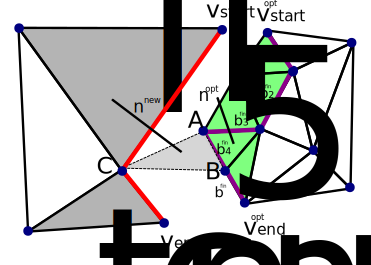
\includegraphics[width=0.15\textwidth]{./img/ch-incr-dens/meshmerge01}&
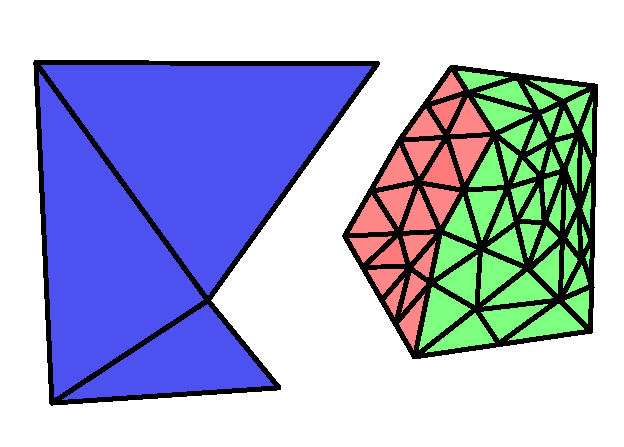
\includegraphics[width=0.15\textwidth]{./img/ch-incr-dens/meshmerge03}&
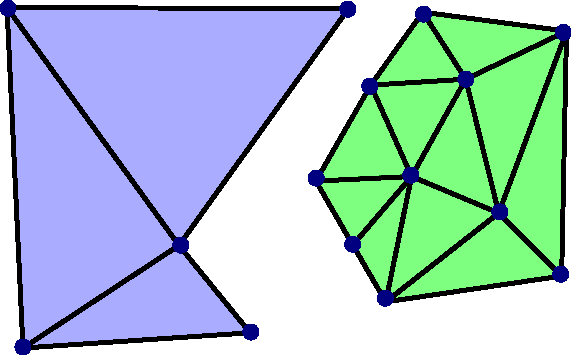
\includegraphics[width=0.15\textwidth]{./img/ch-incr-dens/meshmerge04}&
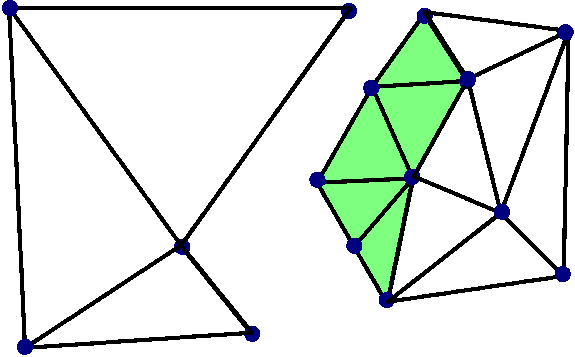
\includegraphics[width=0.15\textwidth]{./img/ch-incr-dens/meshmerge07}&
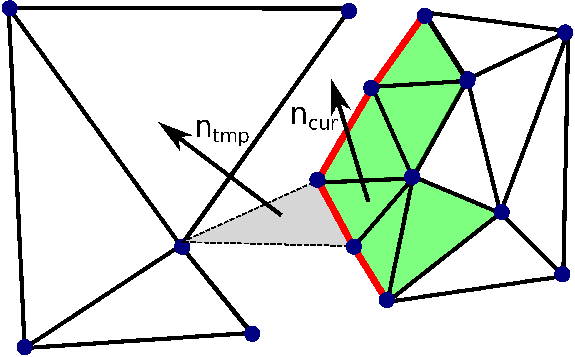
\includegraphics[width=0.15\textwidth]{./img/ch-incr-dens/meshmerge09}&
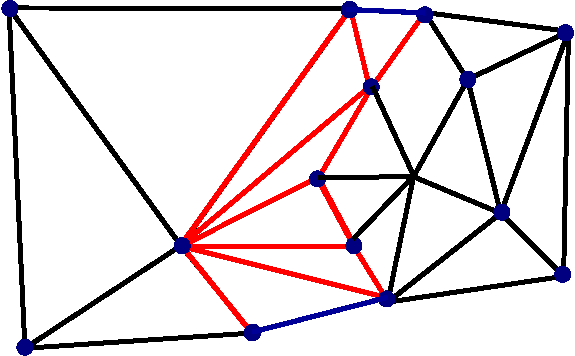
\includegraphics[width=0.15\textwidth]{./img/ch-incr-dens/meshmerge11}\\
(a)&(b)&(c)&
(d)&(e)&(f)\\
\end{tabular}
\label{fig:mesh_merging}
\caption{Mesh merging steps}
\end{figure}
First, we erase all the facets  $f^{\text{rec}} \in \mathit{M}_{0..kW}^{\text{rec}}$ close to $f^{\text{opt}} \in \mathit{M}_{0..(k-1)W}^{\text{opt}}$, i.e., all the $f^{\text{rec}}$ whose bounding boxes intersect at least one of the bounding boxes of the facets $f^{\text{opt}}$ (Fig. \ref{fig:mesh_merging}(b) and Fig. \ref{fig:mesh_merging}(c)).
Once the facets have been removed, $\mathit{M}_{0..kW}^{\text{rec}}$ becomes a set of connected components (meshes); we keep the biggest one, named $\mathit{\bar{M}}_{0..kq}^{\text{rec}}$, whose boundary is the ordered set of edges $\mathit{b}^{\text{rec}} = \{b_1^{\text{rec}}, \dots,  b_k^{\text{rec}}\}$.
If the mesh $\mathit{\bar{M}}_{0..kW}^{\text{rec}}$ is smaller than a threshold $\tau_{bm}=30\%$, it means that the overlapping is predominant and we stop the merging process, keeping the refined mesh as output.

%Then, we define a second ordered set of edges $\mathit{b}^{\text{opt}} = \{b_1^{\text{opt}}, \dots,  b_k^{\text{opt}}\}$ belonging to  $\mathit{M}_{0..t}^{\text{opt}}$ such that the facets we will add to join the two edges, will likely preserve the manifoldness.
Otherwise, we define the set of facets $\hat{f}^{\text{opt}}$ near to $\mathit{b}^{\text{rec}}$, as the intersection among  $k^{bound}$ times the bounding boxes around the facets adjacent to  $\mathit{b}^{\text{rec}}$ and the bounding boxes of $f^{\text{opt}}$  (green faces and their adjacent edges in Fig. \ref{fig:mesh_merging}(d)).
Now, let  $v_{\text{start}}^{\text{opt}}$ and $v_{\text{end}}^{\text{opt}}$ be the two vertices nearest to the extremity of  $\mathit{b}^{\text{rec}}$. 
We define $\mathit{b}^{\text{opt}}$ as the path from $v_{\text{start}}^{\text{opt}}$ to $v_{\text{end}}^{\text{opt}}$ among the edges of the facets in $\hat{f}^{\text{opt}}$ which minimizes the energy:
\begin{equation}
  E_{\text{path}}(b^{\text{opt}}) = \angle (\overrightarrow{n}_b^{\text{opt}},\overrightarrow{n}^{\text{opt-rec}})
\end{equation}
where $\overrightarrow{n}_b^{\text{opt}}$ is the normal of the facet belonging to $\mathit{b}^{\text{opt}}$ and adjacent to  $b^{\text{opt}}$; and
$\overrightarrow{n}^{\text{opt-rec}}$ is the normal of the facet defined by the two vertices $A$ and $B$, extremity of current edge ${b}^{\text{opt}}$ and the nearest vertex in the border $\mathit{b}^{\text{rec}}$ to the vertices $A$ and $B$.
We minimize $E_{\text{path}}$ with the Dijkstra algorithm  (Fig. \ref{fig:mesh_merging}(e)).

Finally we connect the corresponding extremities of the two borders $\mathit{b}^{\text{rec}}$ and $\mathit{b}^{\text{opt}}$, and we create the joining facets by filling the polyline hole with the algorithm of \cite{liepa2003filling}  (Fig. \ref{fig:mesh_merging}(f)).

To update the topology of the mesh, if it changes, we iterate this process for all the boundaries of the mesh  $\mathit{\bar{M}}_{0..kW}^{\text{rec}}$, not negligible, i.e., smaller than $\tau_{\text{top}}= 15\%$ the biggest boundary.



\section{Experimental Evaluation}
\label{sec:exp}
We tested the proposed system in order to stress the flexibility of the approach both for small objects and for large-scale scenes. 
Our algorithm bootstraps from the points, cameras and visibility rays extracted incrementally by openMVG \cite{openMVG}. In Table \ref{fig:expData} we list the features of each dataset, and the statistics of the reconstruction: number of reconstructed surfaces, number of mesh merging and window size, which is chosen to stress the iterative nature of the proposed algorithm.
We performed the experiments on a 4 Core i7-920 CPU at 2.6Ghz (8M Cache), with 24GB of DDR3 SDRAM and a GPU Nvidia GT630M.


\begin{table}[t]
\footnotesize
\centering
  \caption{Output statistics on the two datasets.}
  \label{fig:expData}
\begin{tabular}{lccccc}
&num. cameras& resolution&num. facets& num. merged &$W$ \\
\hline
dinoRing&48&640x480&$\sim$127K&3&15\\
castle P-18&18&3072x2048&$\sim$4.7M&3&5\\
\end{tabular}
\end{table}

In the first experiment, we tested our approach with the \emph{dinoRing} dataset  from the Middelbury evaluation proposed in \cite{seitz2006comparison}. 
The dataset is composed by 48 images with a resolution of 640x480px; in Table \ref{tab:dinoRes} we listed the comparison with the top ranked algorithm \cite{savinov2016semantic}, which is voxel-based, together with the other mesh-based algorithm closer to our proposal.
Our algorithm reaches the less accurate result, but  the output is comparable with the batch state-of-the art algorithm, despite two big restrictions we are forced to work with.
First, our algorithm is the only technique  which estimate incrementally the surface; it considers the images as a sequence and compares only subsequent images, i.e., image $k$ with image $k-1$.
Second, we cannot exploit any silhouette information, and the visuall hull, since it cannot be estimated in general scenes.
Fig. \ref{fig:dinoIncr} illustrates the incremental reconstruction of dino: the red circles underlines the topology change handled by our novel mesh merging algorithm.

\begin{table}[t]
\scriptsize
\centering
  \caption{Results on dinoRing dataset.}
  \label{tab:dinoRes}
\begin{tabular}{lccccccc}
%method & Accuracy (mm) &Completeness (\%)\\
\hline
&Savinov\cite{savinov2016semantic}&DCV\cite{li2015detail}&Zarahescu\cite{zaharescu2007transformesh}&Vu\cite{hiep2009towards}&SurfEvolution&Gargallo\cite{gargallo2007minimizing}&proposed\\
&(batch)&(batch)&(batch)&(batch)&(batch)&(batch)&(incremental)\\
Accuracy (mm) &0.25&0.28&0.42&0.53&0.56&0.6&1.27\\
Comp. (\%)&99.9&100&98.6&99.7&97.7&92.9&87.8
\end{tabular}
\end{table}



 \begin{figure}[t]
  \centering
  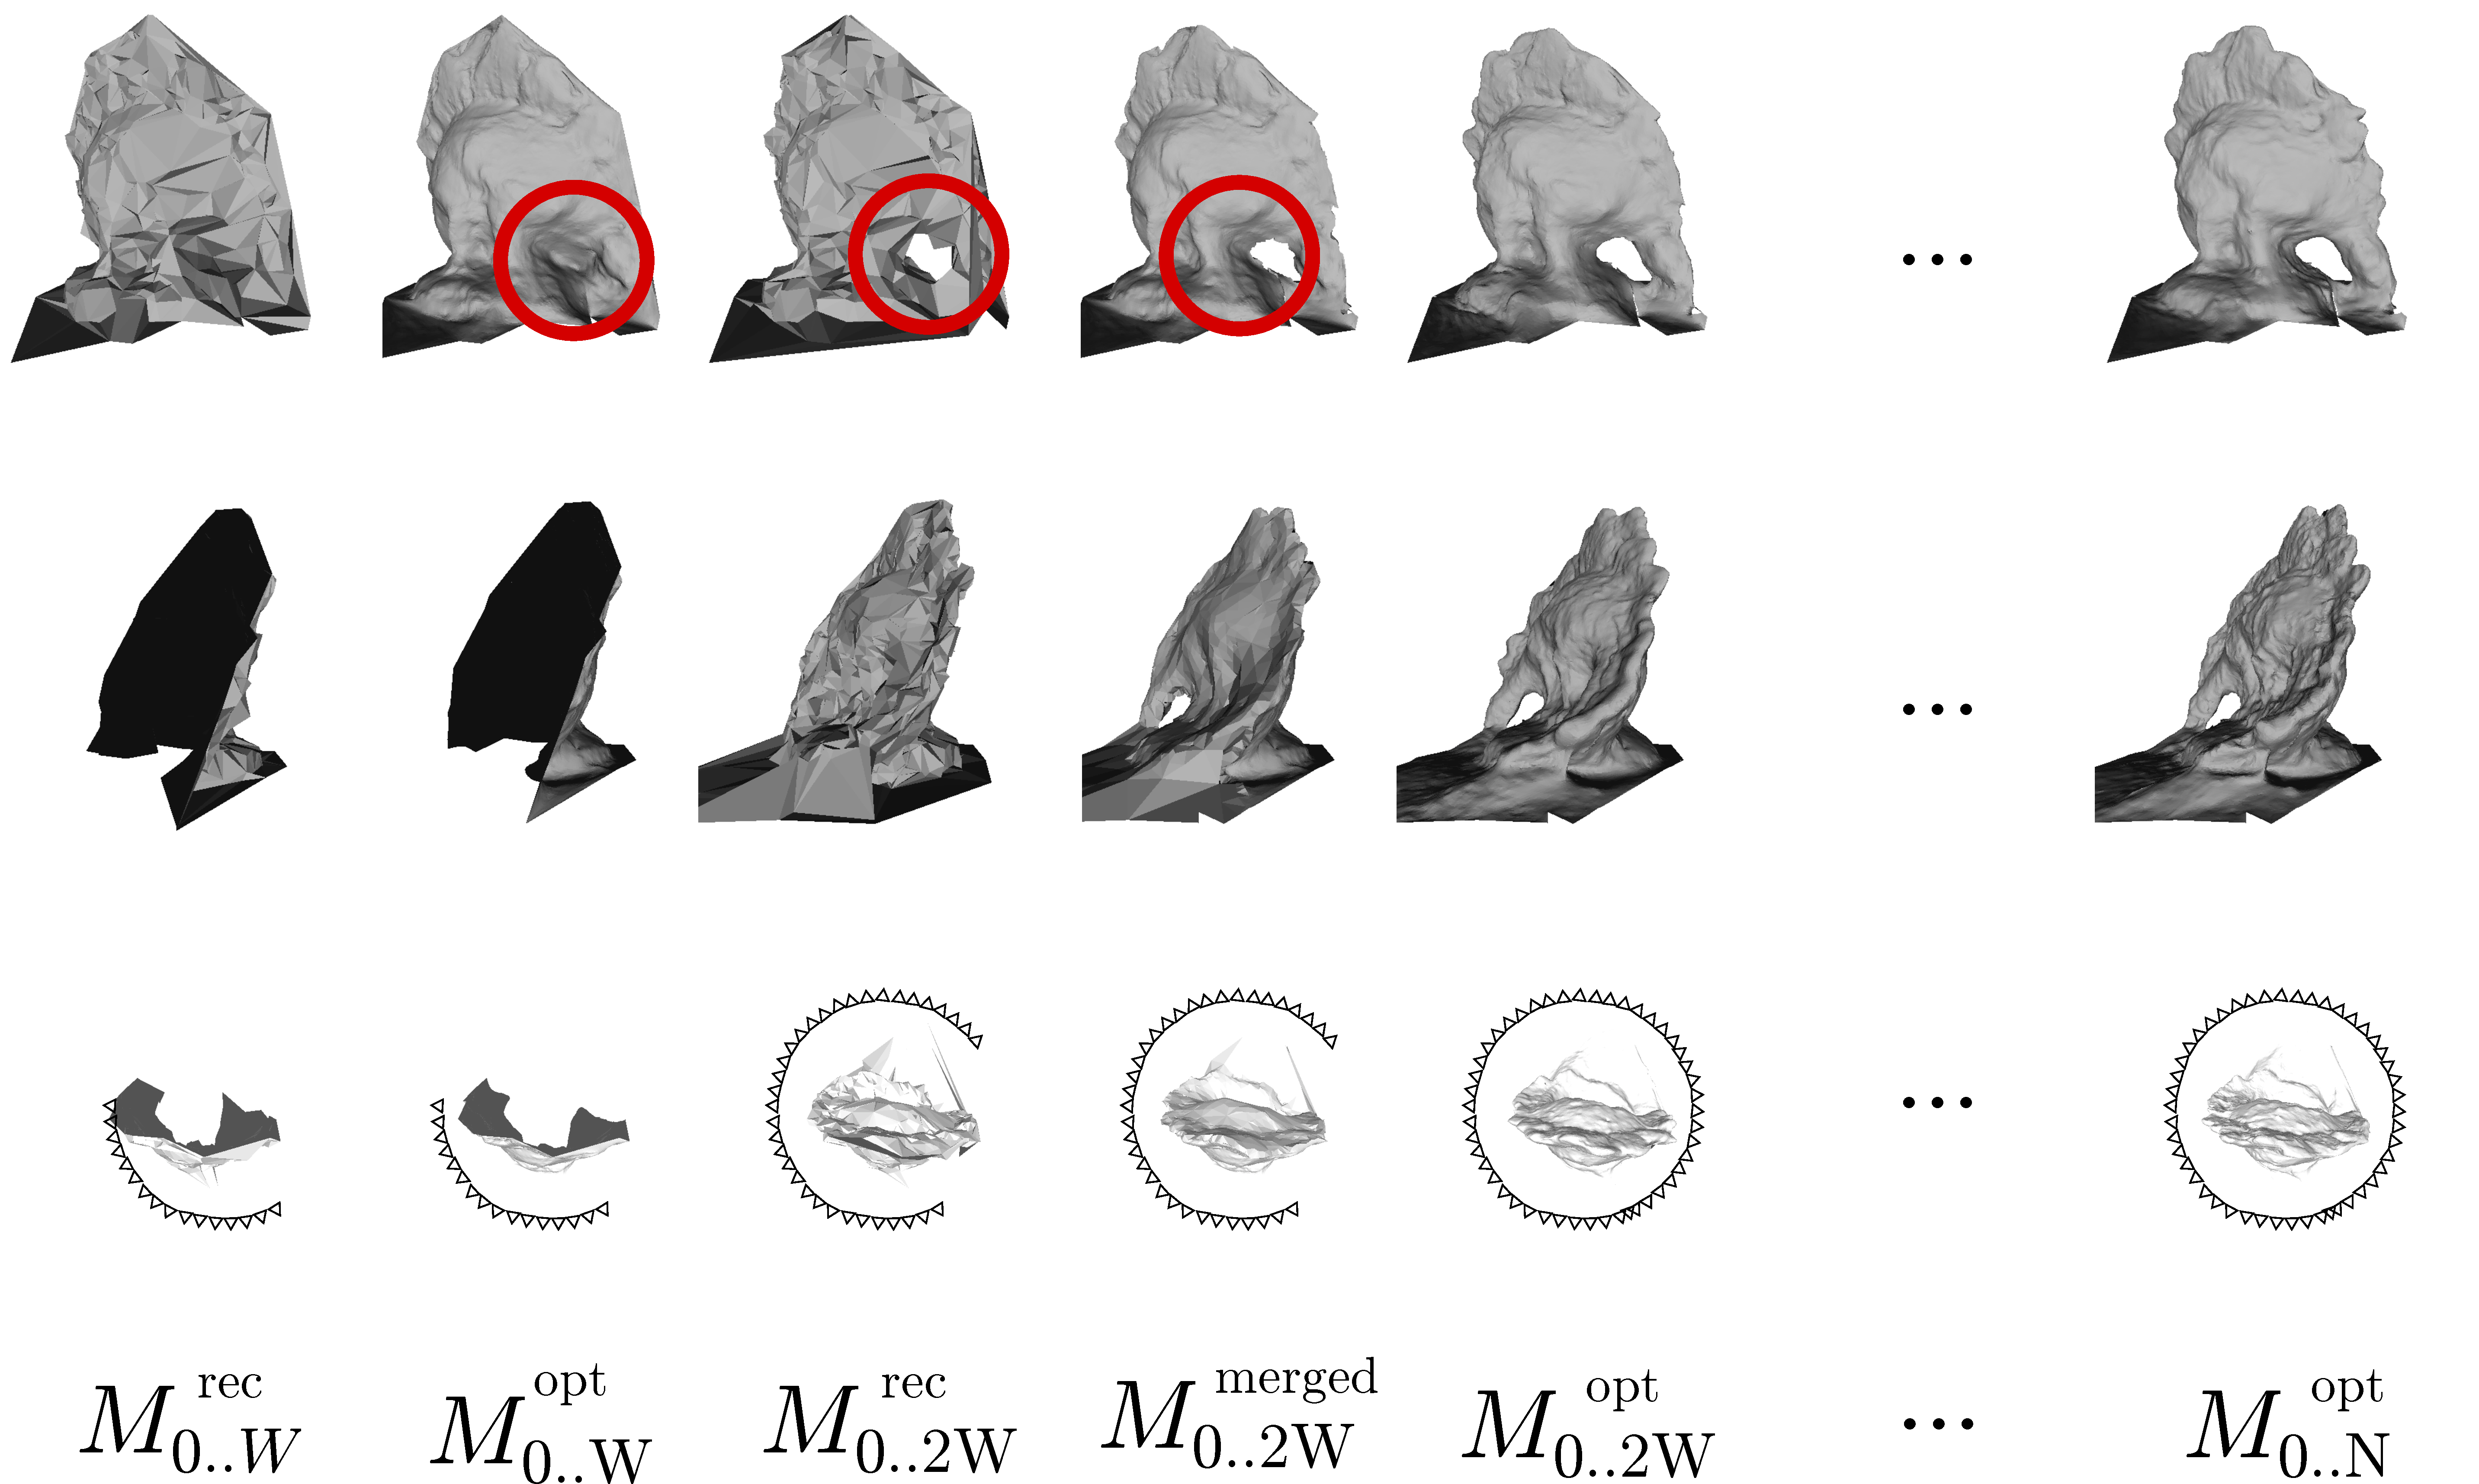
\includegraphics[width=\textwidth]{./img/ch-incr-dens/dino}
  \caption{Incremental reconstruction on the dino dataset.}
  \label{fig:dinoIncr}
\end{figure}


Then we experimented our approach with the \emph{castle-P18} dataset provided in \cite{strecha2008}: no ground truth is available, but is the only sequence of the dataset able to show the incremental behaviour of our approach, since subset of cameras observe parts of the scene. 
The Fig. \ref{fig:castle} shows the results, and Fig. \ref{fig:detailcastle} displays a detail of the reconstruction before and after the refiement. The final reconstruction is accurate  an detailed, especially with respect to the initial rough mesh.
Let notice in Table \ref{fig:expData} that the number of the reconstructed facet is huge, but all the computations have been performed in the memory without the need to dump any data on disk. Indeed the volumetric stage of our algorithm, i.e., the incremental manifold reconstruction, extracts only a  simplified mesh, which is successively refined relying on a mesh-based representation.



\begin{figure}[t]
\centering
\begin{tabular}{cc}
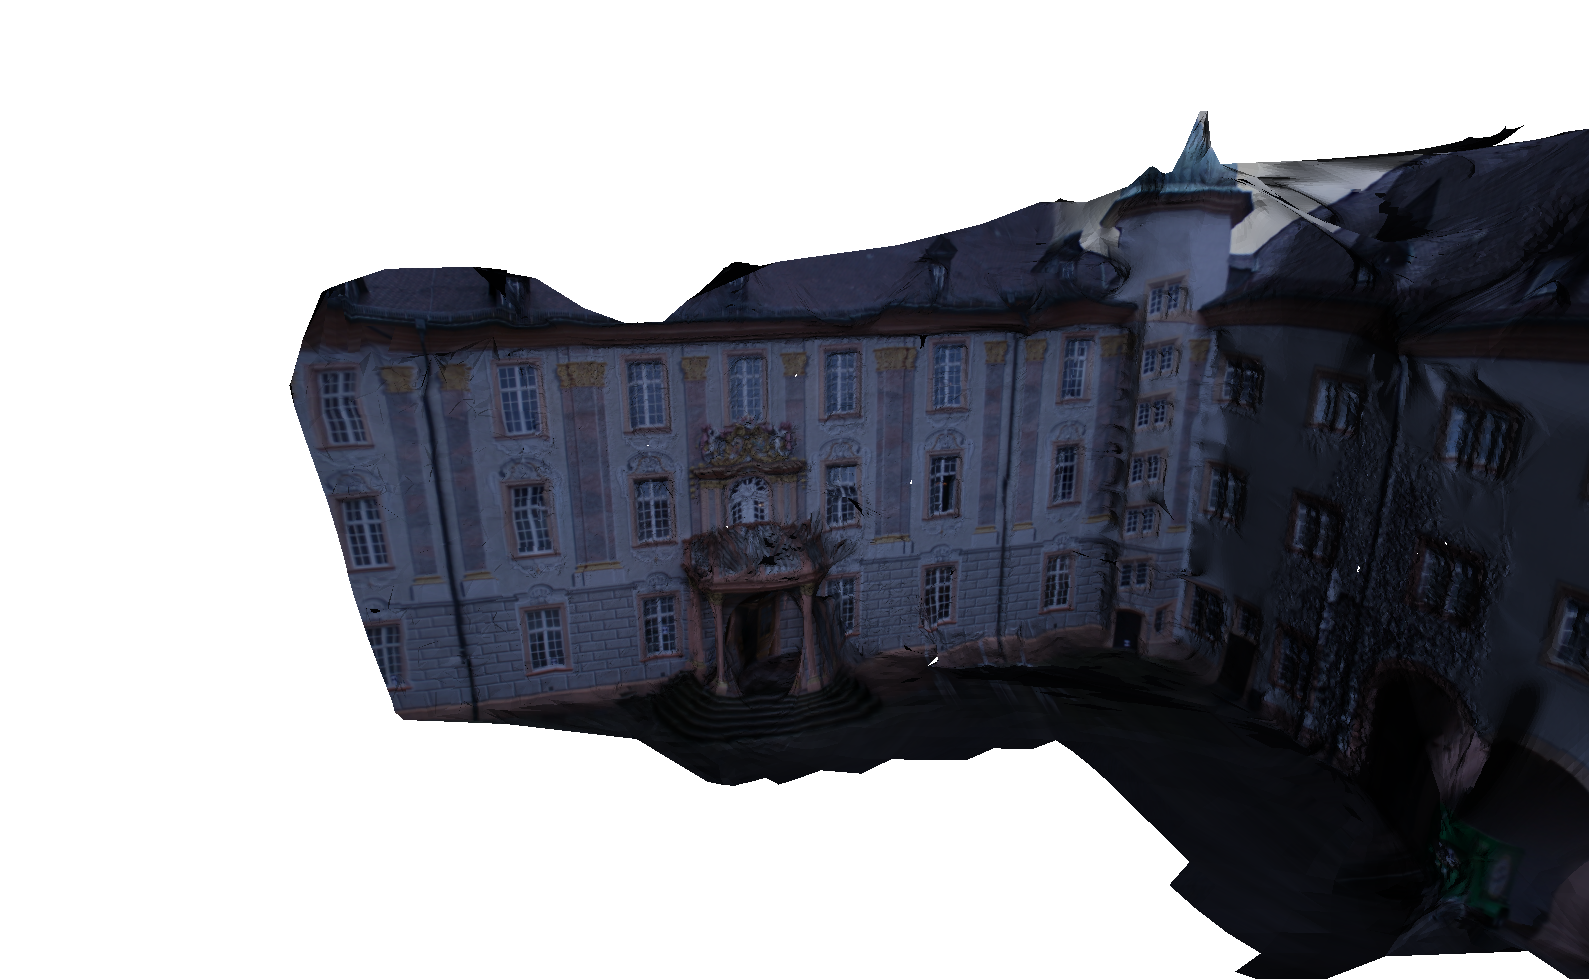
\includegraphics[width=0.35\textwidth]{./img/ch-incr-dens/castle01}&
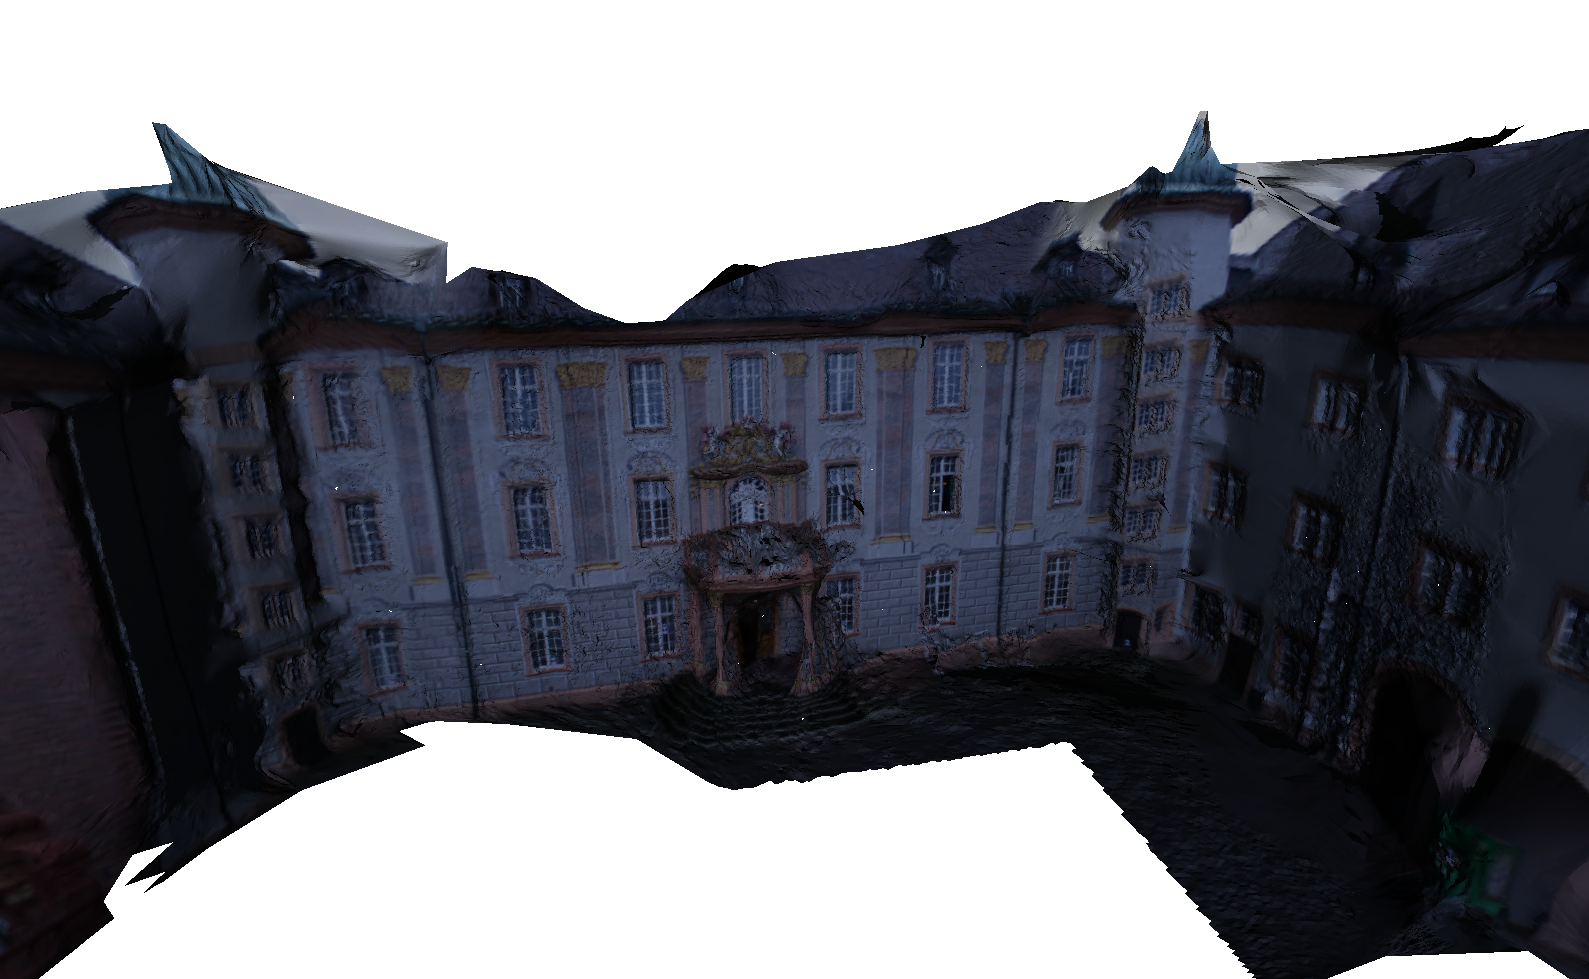
\includegraphics[width=0.35\textwidth]{./img/ch-incr-dens/castle02}\\
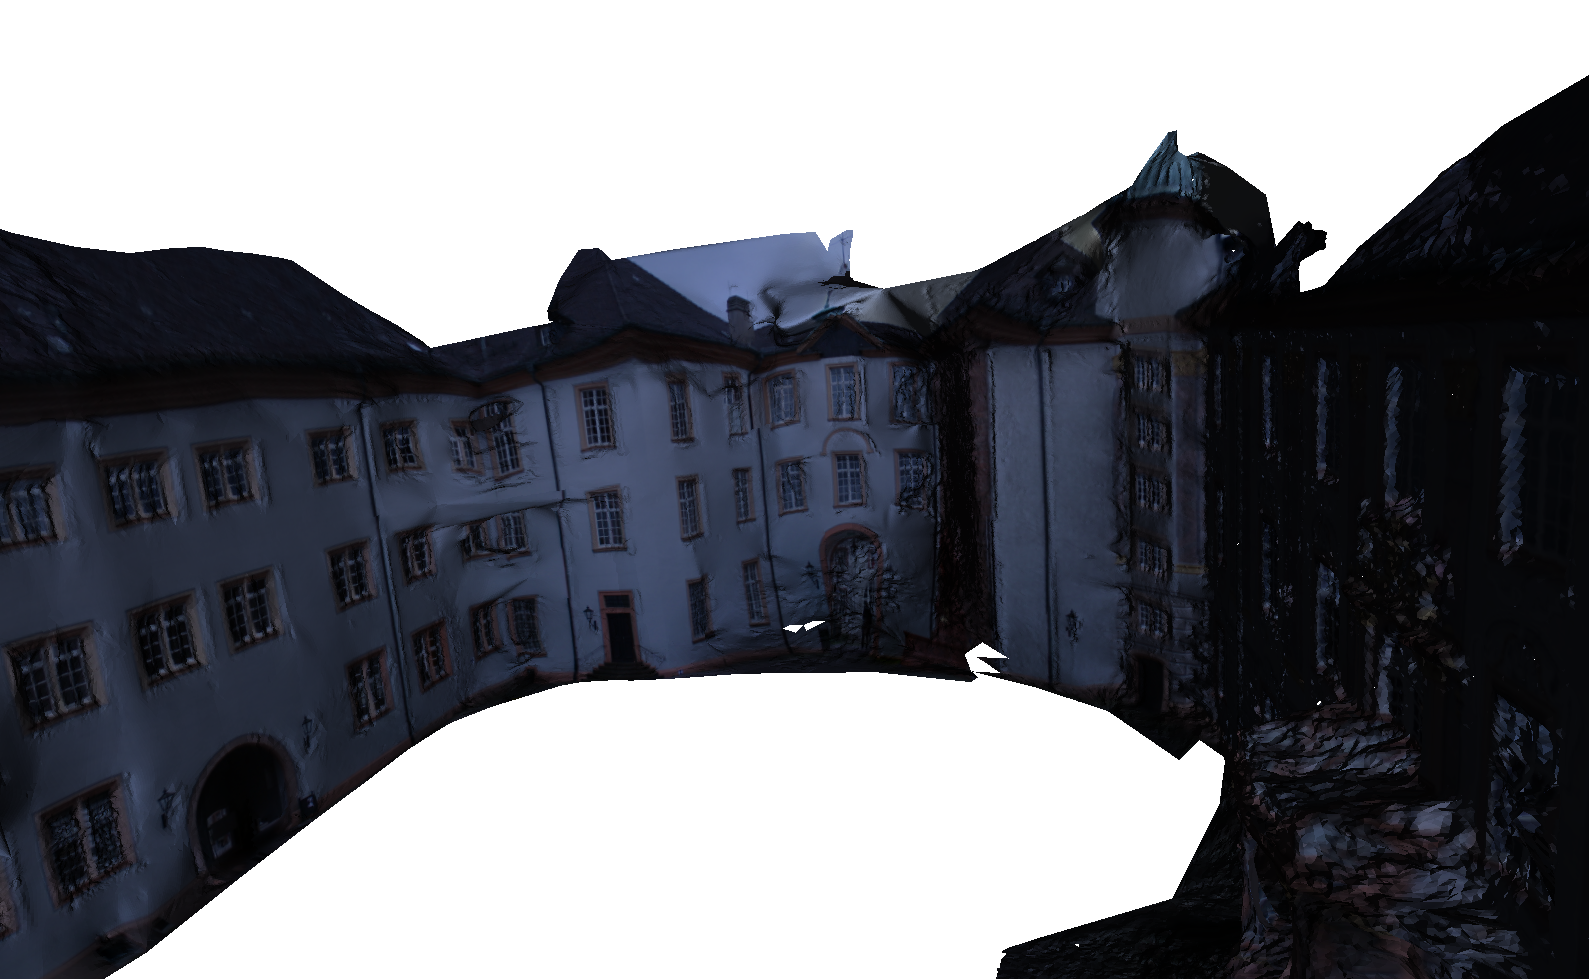
\includegraphics[width=0.35\textwidth]{./img/ch-incr-dens/castle03}&
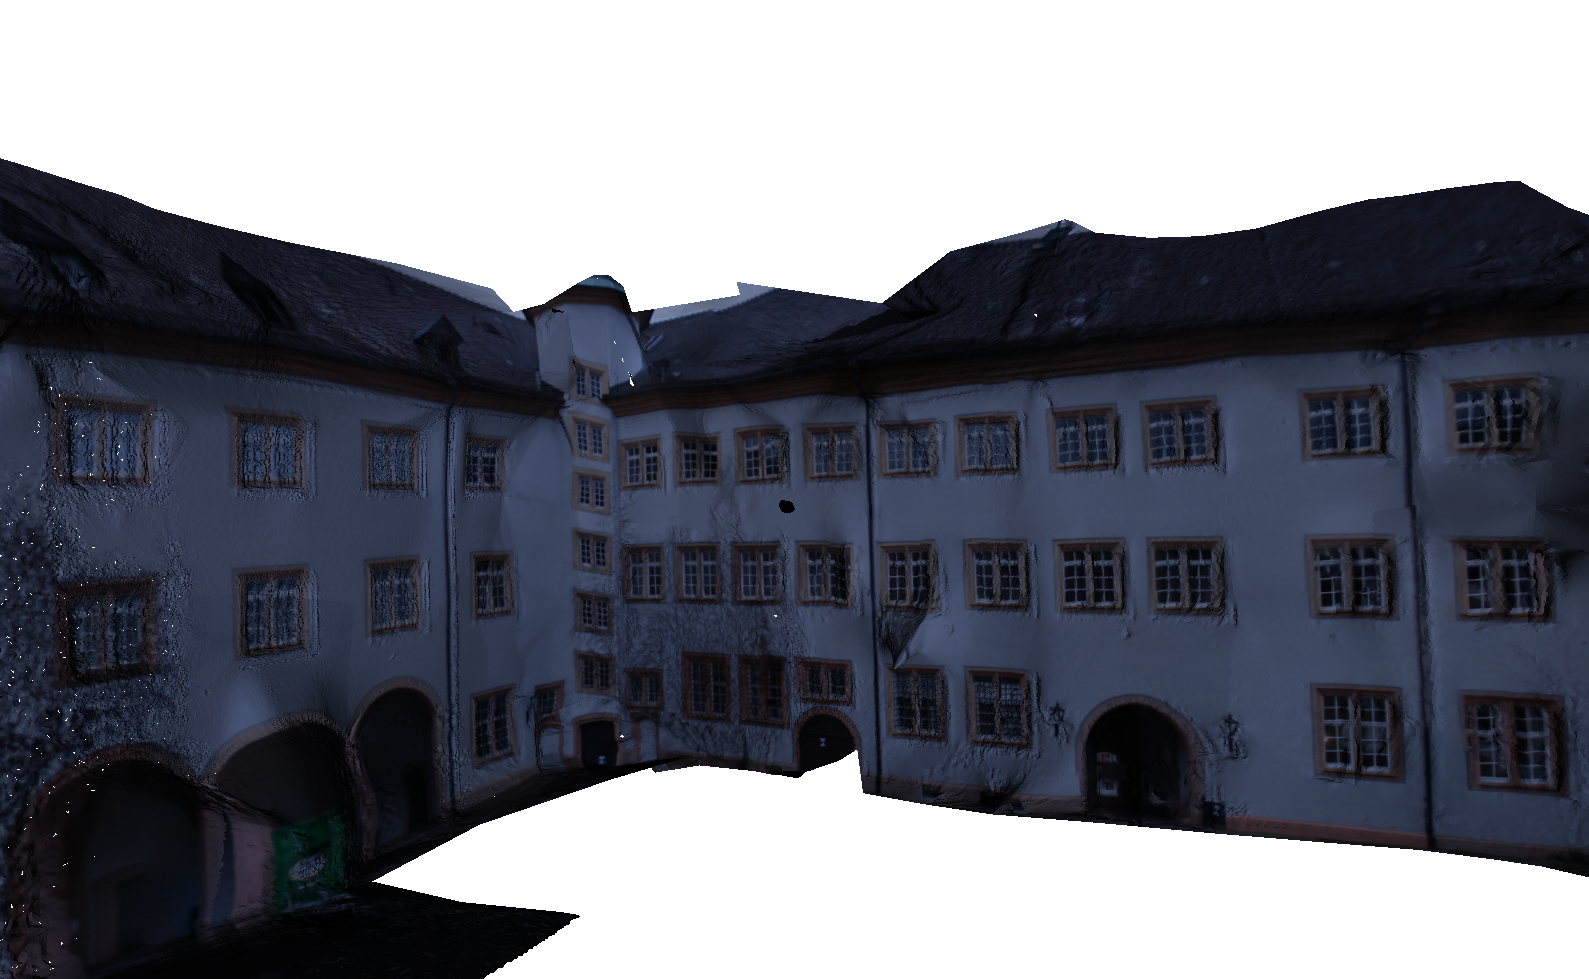
\includegraphics[width=0.35\textwidth]{./img/ch-incr-dens/castle04}
\end{tabular}
\label{fig:castle}
\caption{Incremental reconstruction of \emph{castle-P18} dataset}.
\end{figure}

\begin{figure}[tpb]
\centering
\begin{tabular}{cc}
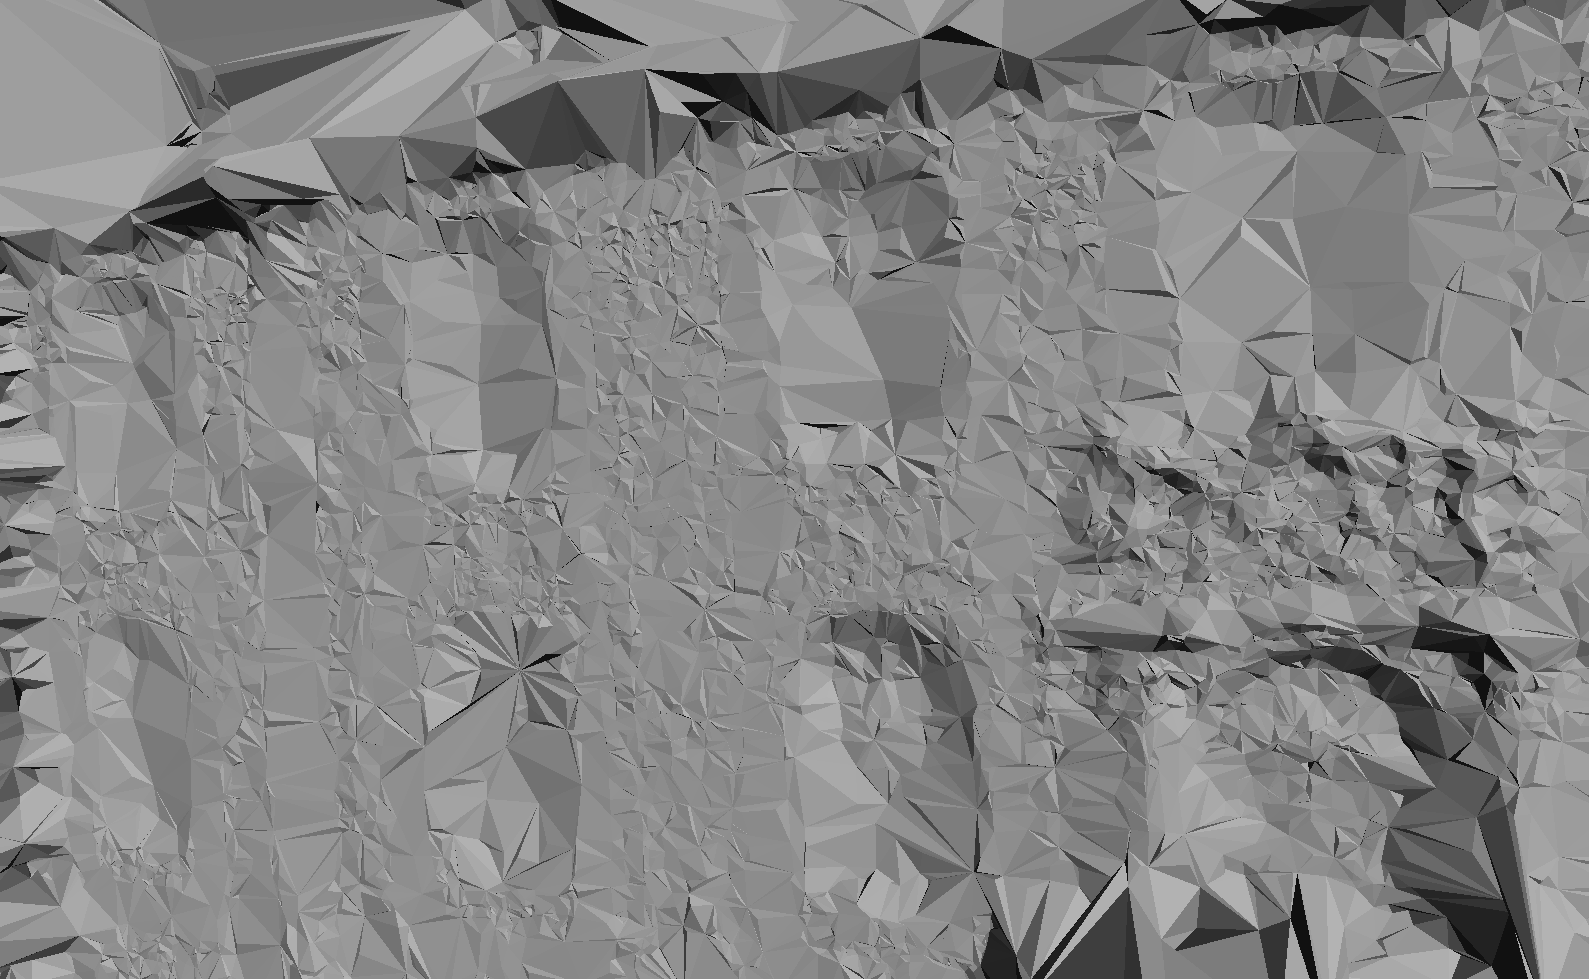
\includegraphics[width=0.4\textwidth]{./img/ch-incr-dens/castle12}&
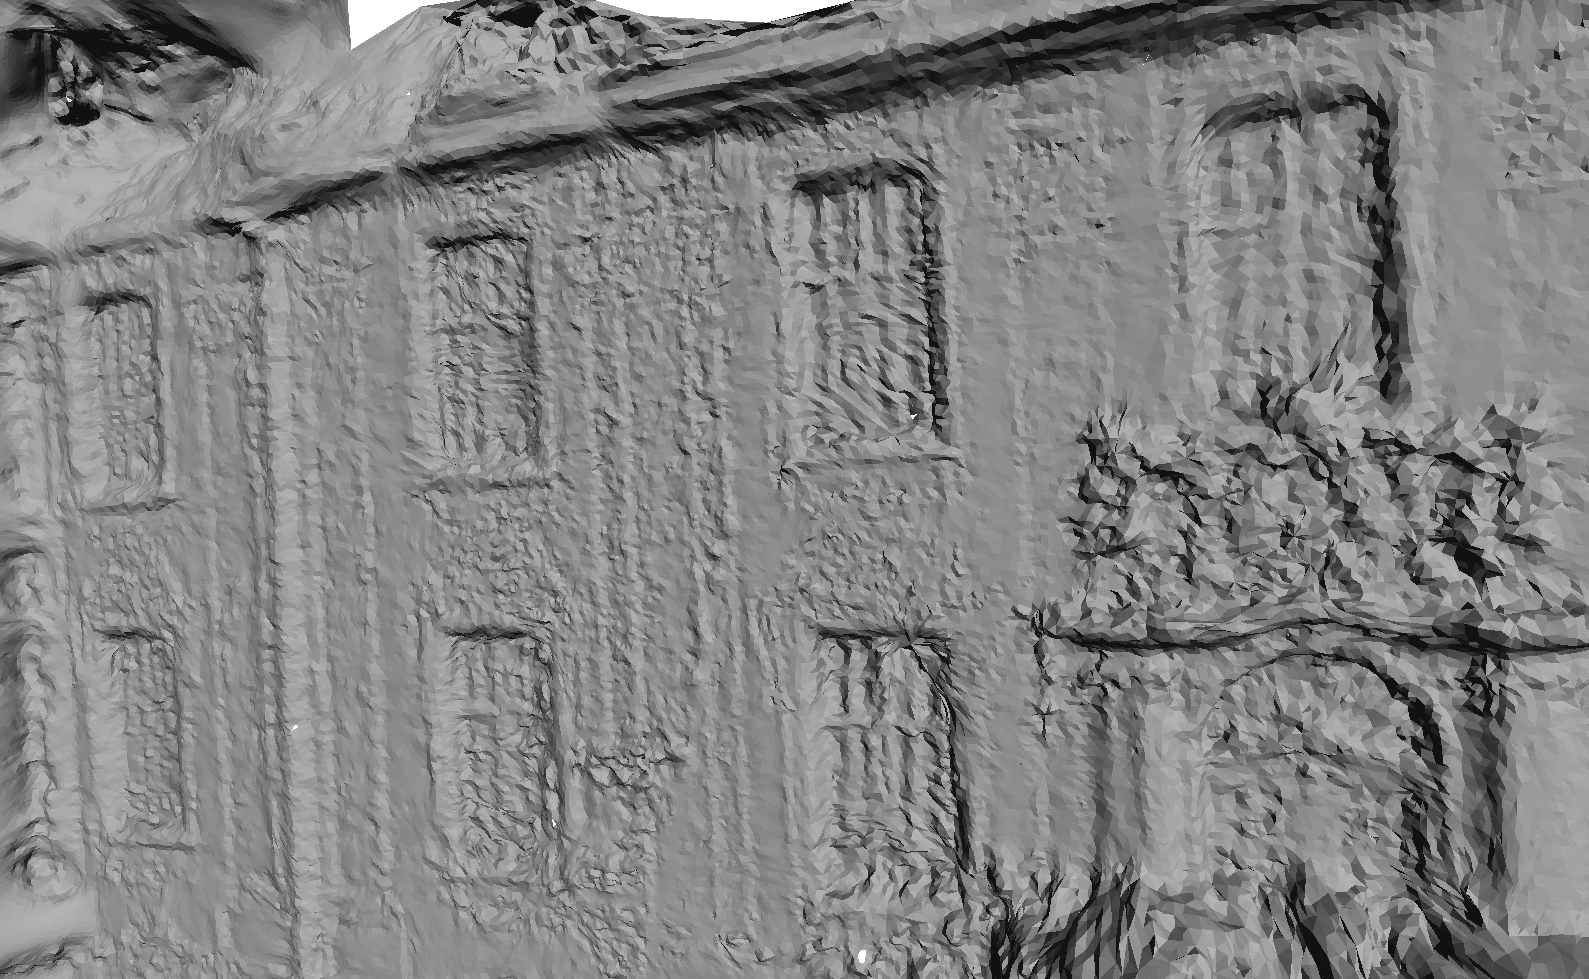
\includegraphics[width=0.4\textwidth]{./img/ch-incr-dens/castle11}\\
(a)&(b)
\end{tabular}
\label{fig:detailcastle}
\caption{Detail of Castle reconstruction before (a) and after(b) the photo-metric refinement}.
\end{figure}





